\section{Generative Adversarial Networks}
In 2014, Ian Goodfellow invented Generative Adversarial Networks (GANs). The concept is rather simple, as it consists of two competing networks. The first network is called a generator and creates new images based on an input image. Here, for consistency, the images generated by the generator will be denoted as generated images. The second network is the discriminator, which tries to distinguish between the generated image (predicted image) and the real image (ground truth) \citep{goodfellow2014generative}.
As a consequence of training both networks alternately, the generated images eventually become indistinguishable from the real images. It is nothing more than a two-player min-max game, a famous problem in game theory. GAN was initially proposed in the formulation form as:
\begin{equation}
	\centering
	\begin{aligned}
		\min_{G} \max_{D} V(D, G) &= \mathbb{E}_{x \sim p_{data}(x)} \left[ \log D(x) \right] \\
		&+ \mathbb{E}_{z \sim p_{z}(z)} \left[ \log \left( 1-D(G(z)) \right) \right]
	\end{aligned}
	\label{eq:Basic_GAN}
\end{equation}
here, $V(D, G)$ is the value function of the min-max game. 

The goal is now to learn the distribution of the generator $p_g$ over the data $x$. We have input noise variables $p_z(z)$, as well as the two perceptrons $G(z; \theta_g)$ and $D(x; \theta_d)$ with parameters $\theta_i$. $G$ represents a differential function that maps from $z$ to the data space $x$, while $D(x)$ represents the probability that $x$ is from the real data \citep{goodfellow2014generative}. The problem can be reformulated as: 
\begin{equation}
	\centering
	\begin{aligned}
		\max_{D} V(G, D) &= \mathbb{E}_{x \sim p_{data}} \left[ \log D^{*}_{G}(x) \right] \\ 
		&+ \mathbb{E}_{x \sim p_{g}} \left[ \log \left( 1 - D^{*}_{G}(x) \right) \right]
	\end{aligned}
	\label{eq:GAN_reformulated}
\end{equation}
where $D^{*}_{G}$ denotes the optimum of the discriminator for a given fixed generator and is expressed as
\begin{equation}
	\centering
	D^*_G(x) = \frac{p_{data}(x)}{p_{data}(x) + p_g(g)}
	\label{eq:Disc_optimum}
\end{equation}
It can now be shown that the global optimum of equation (\ref{eq:GAN_reformulated}) is reached if and only if $p_g = p_{data}$. Furthermore, if both $G$ and $D$ are allowed to reach their optima, $p_g$ converges to $p_{data}$. A more detailed discussion of the problem, including proofs, can be found in \citep{goodfellow2014generative}.
\begin{figure}
	\centering
	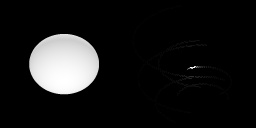
\includegraphics[width=\linewidth]{fig/ellipsoid_0.jpg}
	\caption{Merged image, which includes the original and the sparsely sampled Fourier plane. It is exactly what the GAN receives. }
	\label{fig:GANinput}
\end{figure}
\begin{figure}
	\centering
	\begin{subfigure}{\linewidth}
		\centering
		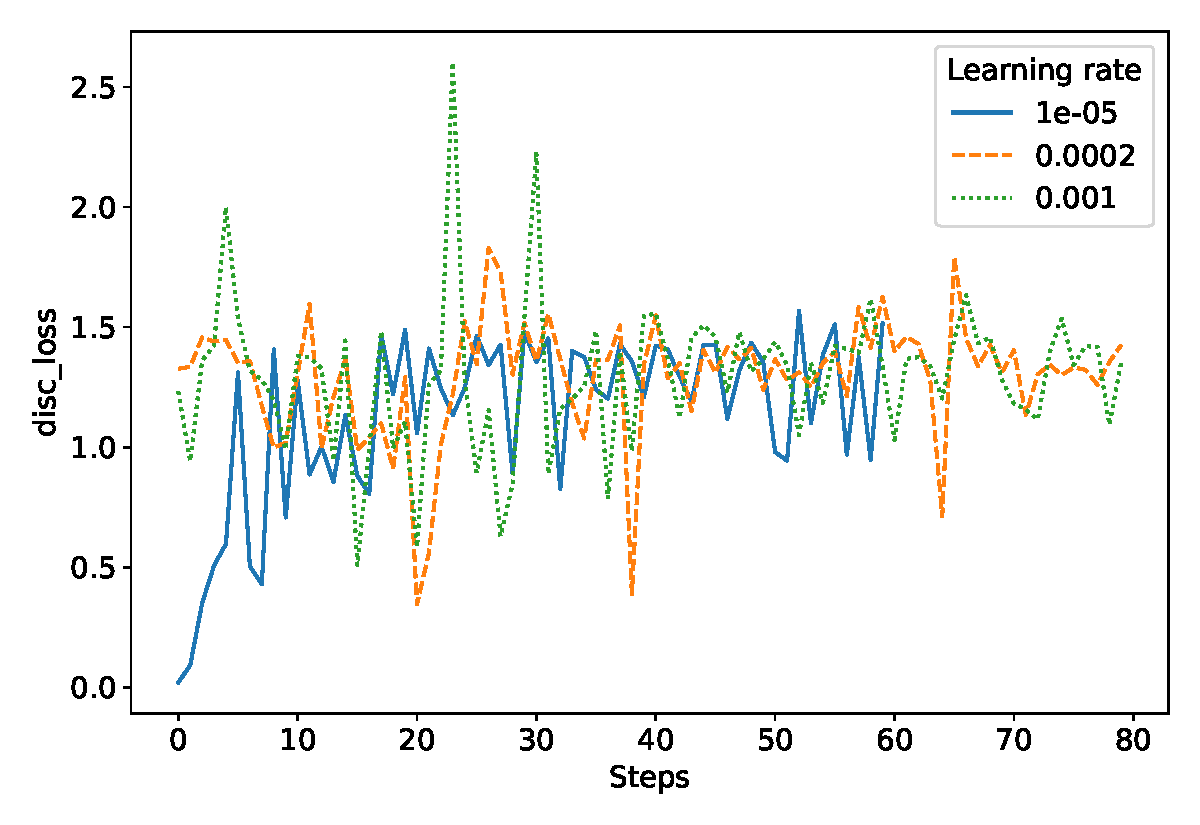
\includegraphics[width=\textwidth]{fig/analysis/Plot_learning_rate_disc_loss.pdf}
		\caption{Discriminator loss for three different learning rates. }
		\label{fig:Plot_learning_rate_discloss}
	\end{subfigure}\hfill
	\begin{subfigure}{\linewidth}
		\centering
		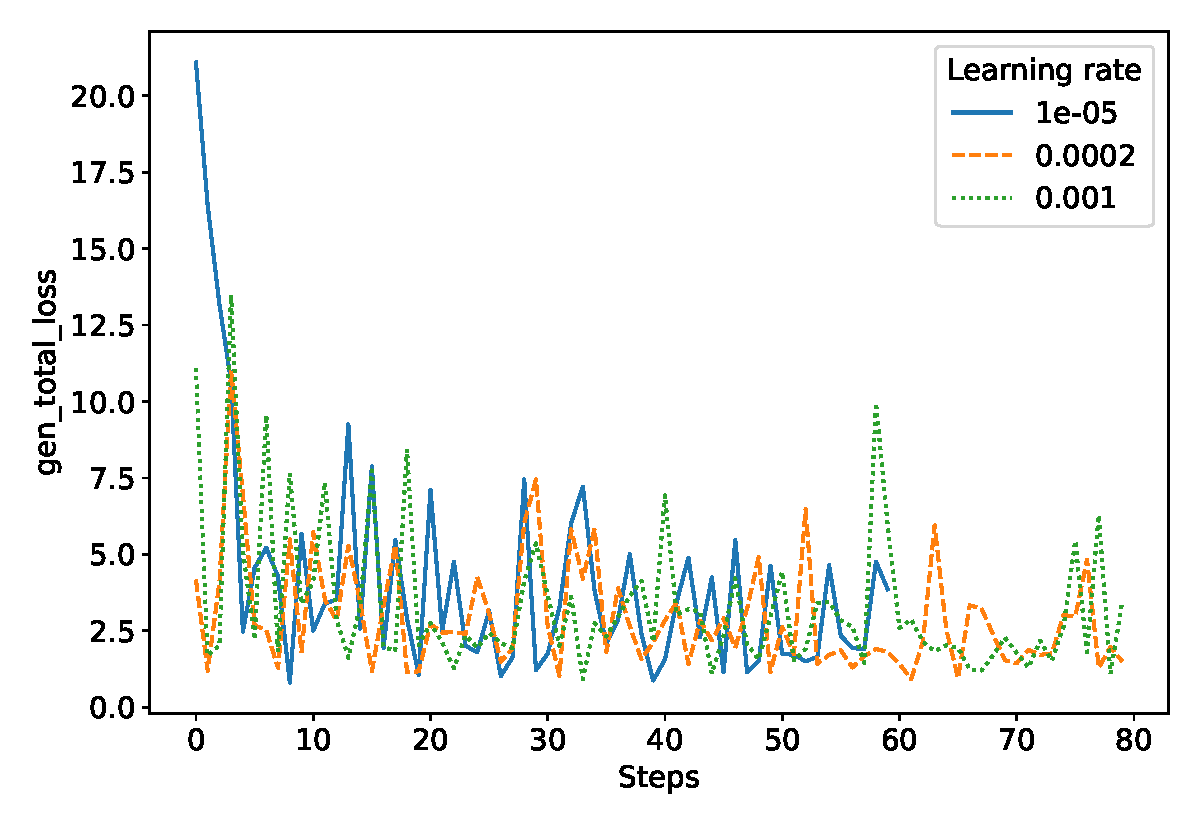
\includegraphics[width=\textwidth]{fig/analysis/Plot_learning_rate_gen_total_loss.pdf}
		\caption{Total generator loss for different learning rates (eqn. (\ref{eq:total_gen_loss})).}
		\label{fig:Plot_learning_rate_genloss}
	\end{subfigure}\hfill
	\caption{Generator and discriminator losses for three different learning rates. The upper figure shows the total discriminator loss, and the lower figure shows the total generator loss. There is no significant difference, but the highest learning rate might be prone to outliers. }
	\label{fig:Plot_learning_rate_loss}
\end{figure}
\begin{figure}
	\centering
	\begin{subfigure}{\linewidth}
		\centering
		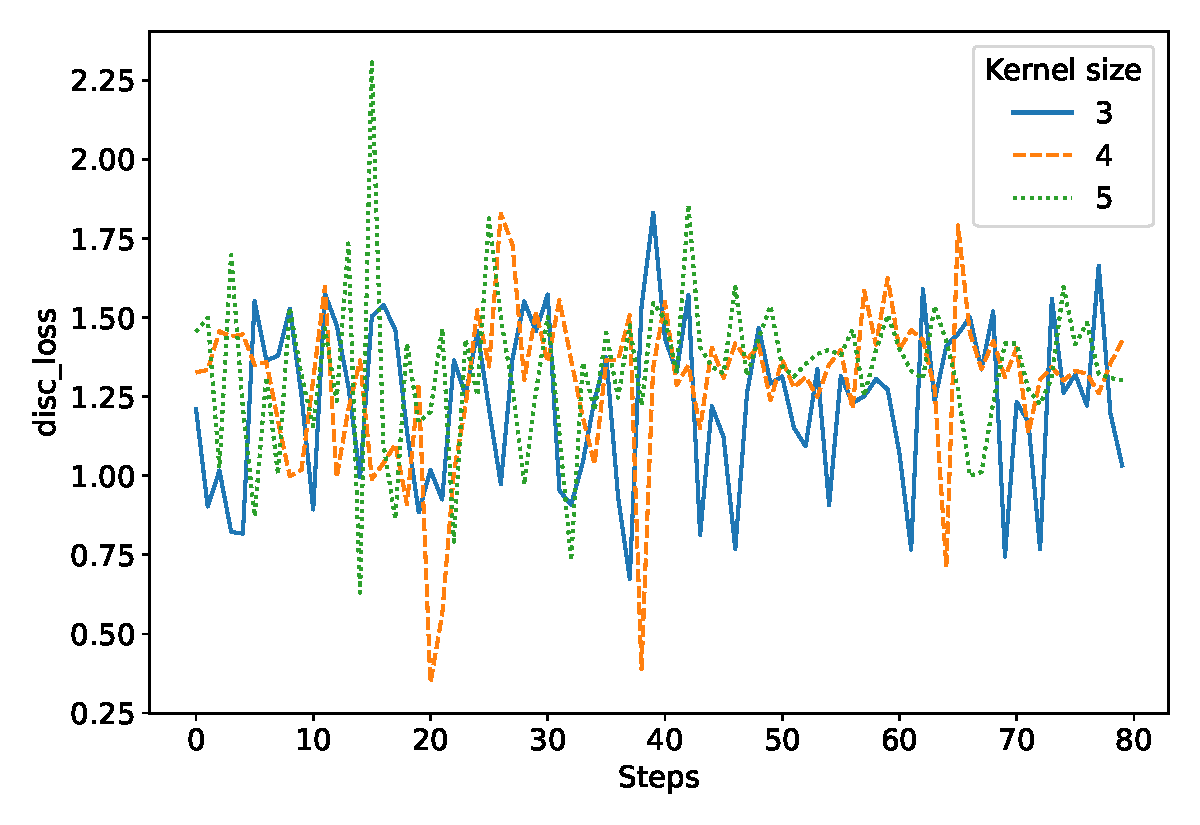
\includegraphics[width=\textwidth]{fig/analysis/Plot_Kernel_size_disc_loss.pdf}
		\caption{Discriminator loss for three different kernel sizes. }
		\label{fig:Plot_kernel_size_discloss}
	\end{subfigure}\hfill
	\begin{subfigure}{\linewidth}
		\centering
		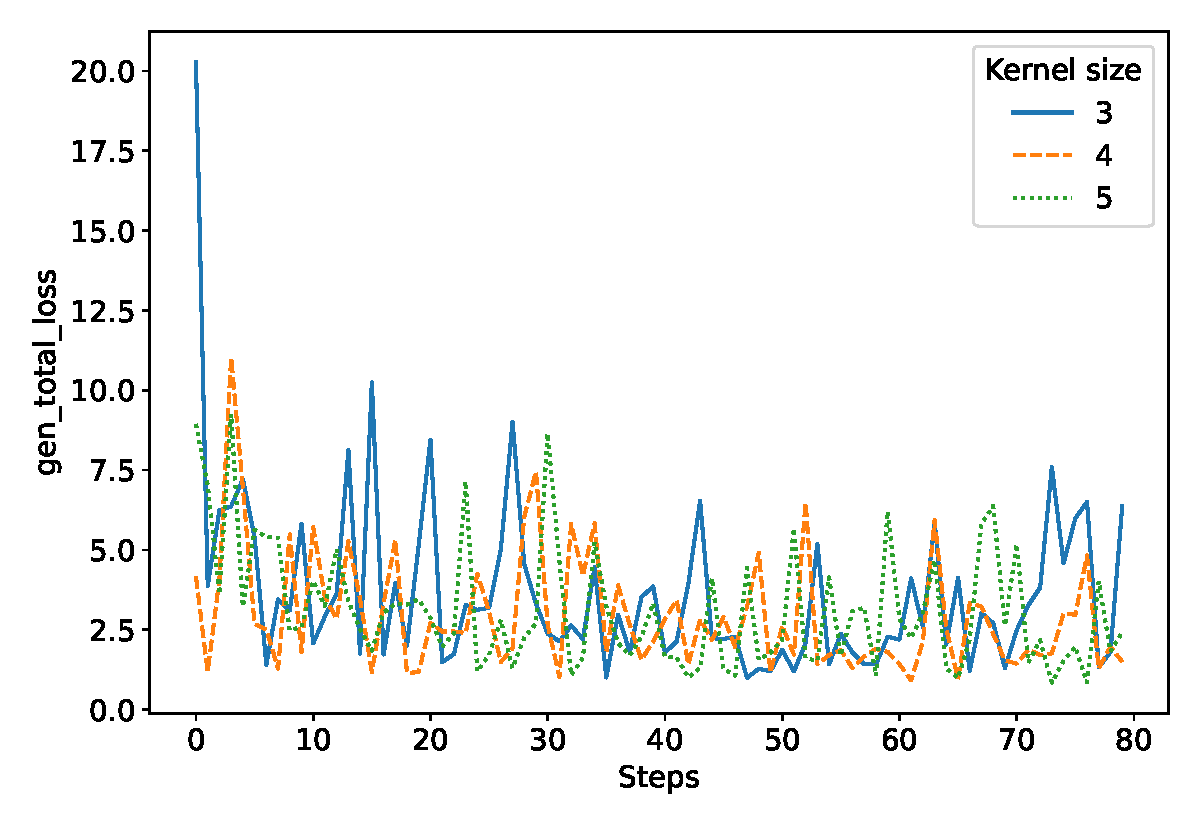
\includegraphics[width=\textwidth]{fig/analysis/Plot_Kernel_size_gen_total_loss.pdf}
		\caption{Total generator loss for three different kernel sizes.}
		\label{fig:Plot_kernel_size_genloss}
	\end{subfigure}\hfill
	\caption{Generator and discriminator losses for three different kernel sizes in the convolutional layers. Here, the smallest kernel size has many outliers, while the largest kernel size seems to be the most stable.}
	\label{fig:Plot_kernel_size_loss}
\end{figure}
\begin{figure*}
	\centering
	\begin{subfigure}{0.5\linewidth}
		\centering
		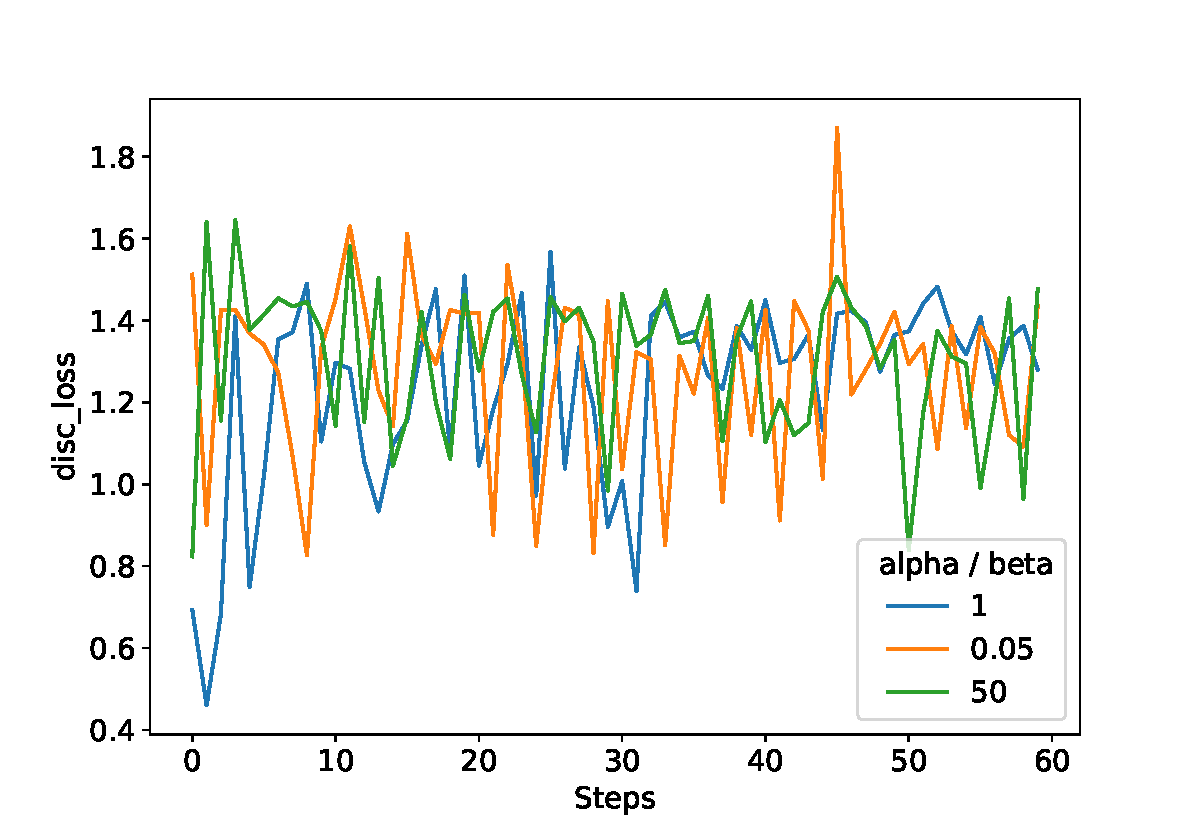
\includegraphics[width=\textwidth]{fig/analysis/Plot_noise_factor_disc_loss.pdf}
		\caption{Discriminator loss for different noise percentages.}
		\label{fig:Plot_noise_discloss}
	\end{subfigure}\hfill
	\begin{subfigure}{0.5\linewidth}
		\centering
		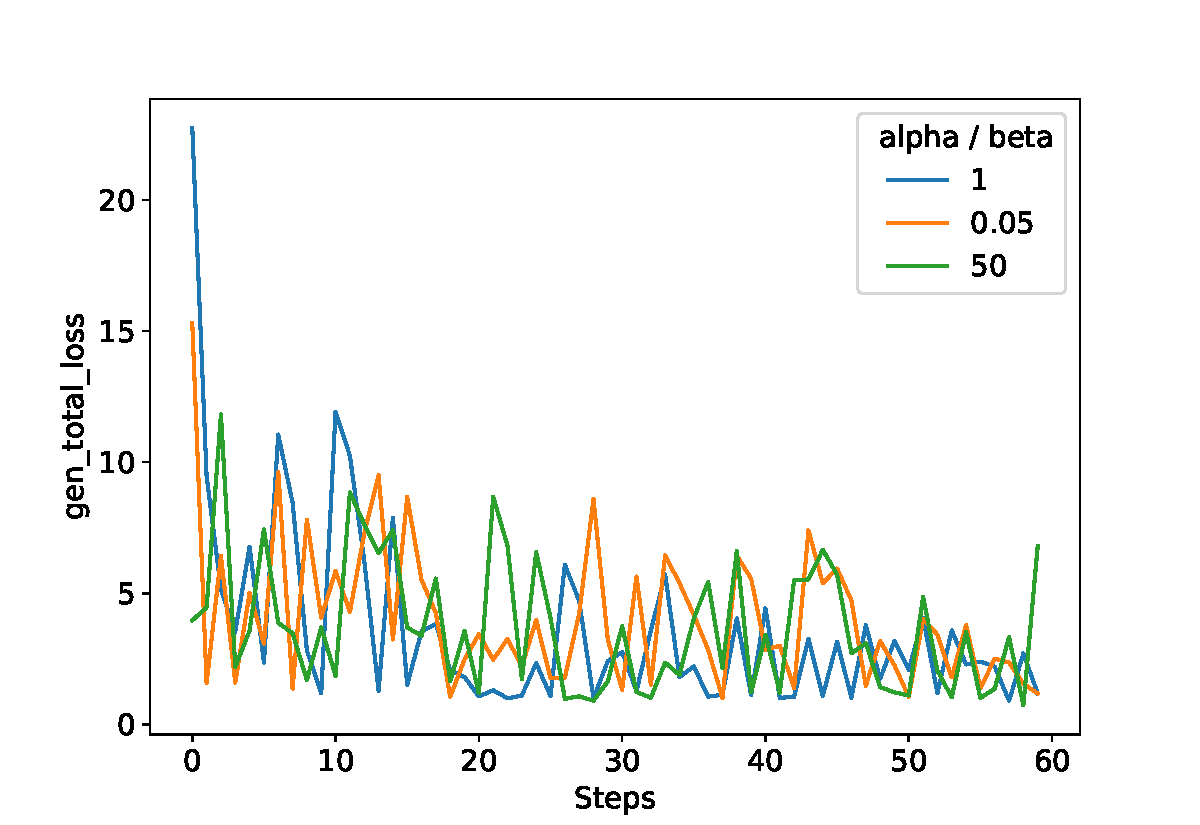
\includegraphics[width=\textwidth]{fig/analysis/Plot_noise_factor_gen_total_loss.pdf}
		\caption{Generator losses for different noise percentages.}
		\label{fig:Plot_noise_genloss}
	\end{subfigure}\hfill
	\caption{Effect of the Salt and Pepper noise introduced in the images. Different ratios between $\alpha$ and $\beta$ are shown. There is no significant effect. Please note that these results are from training on 64-pixel images.}
	\label{fig:Plot_noise_loss}
\end{figure*}
\begin{figure*}
	\centering
	\begin{subfigure}{0.5\linewidth}
		\centering
		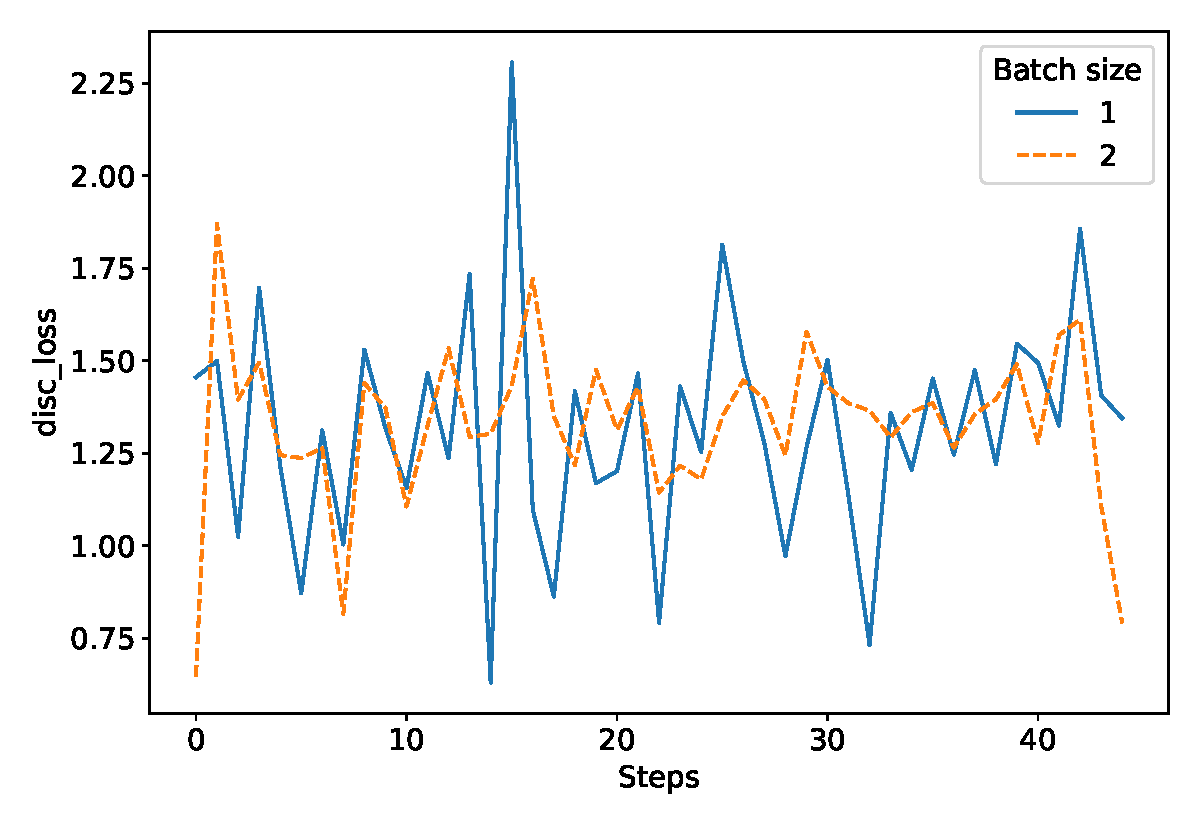
\includegraphics[width=\textwidth]{fig/analysis/Plot_Batchsize_disc_loss.pdf}
		\caption{Discriminator loss for different batch sizes.}
		\label{fig:Plot_batchsize_discloss}
	\end{subfigure}\hfill
	\begin{subfigure}{0.5\linewidth}
		\centering
		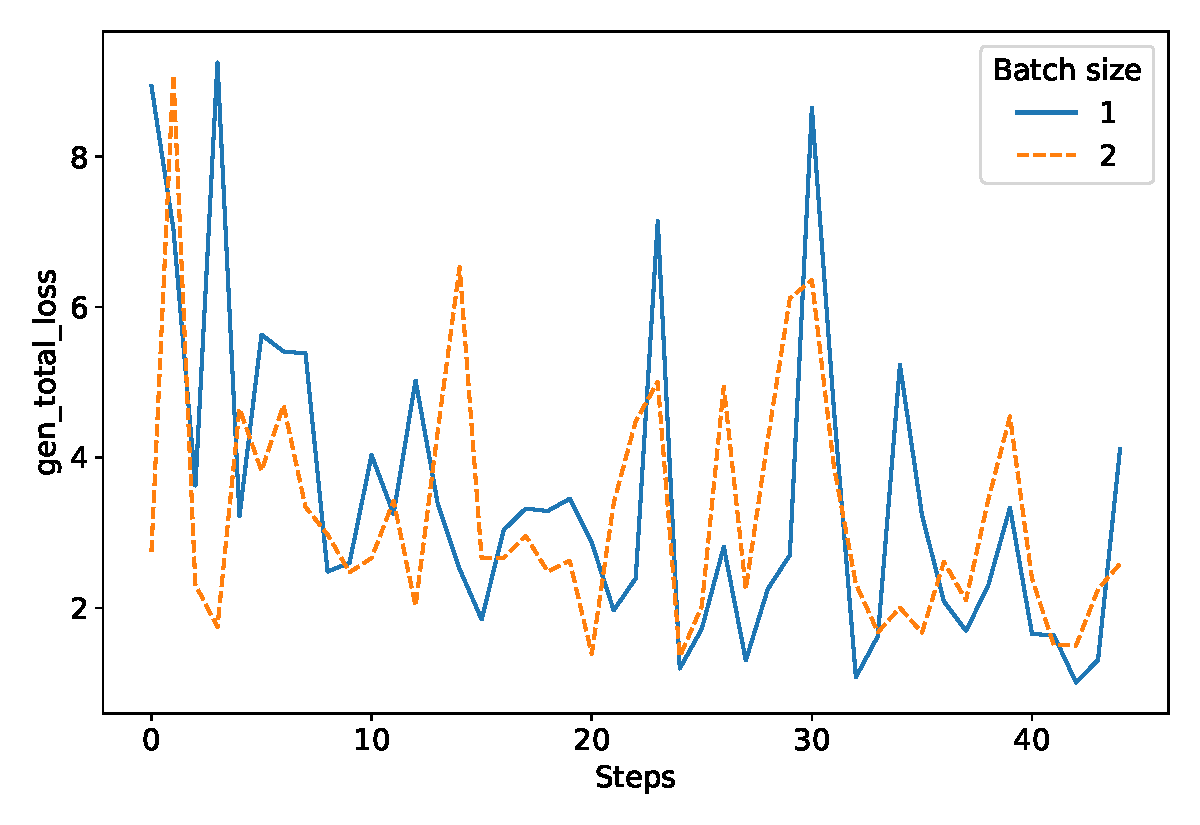
\includegraphics[width=\textwidth]{fig/analysis/Plot_Batchsize_gen_total_loss.pdf}
		\caption{Generator losses for different batch sizes.}
		\label{fig:Plot_batchsize_genloss}
	\end{subfigure}\hfill
	\caption{Loss functions for two different batch sizes. Large batch sizes seem to be more robust, but they also increase training time significantly. }
	\label{fig:Plot_batchsize_loss}
\end{figure*}
\begin{figure*}
	\centering
	\begin{subfigure}{0.5\linewidth}
		\centering
		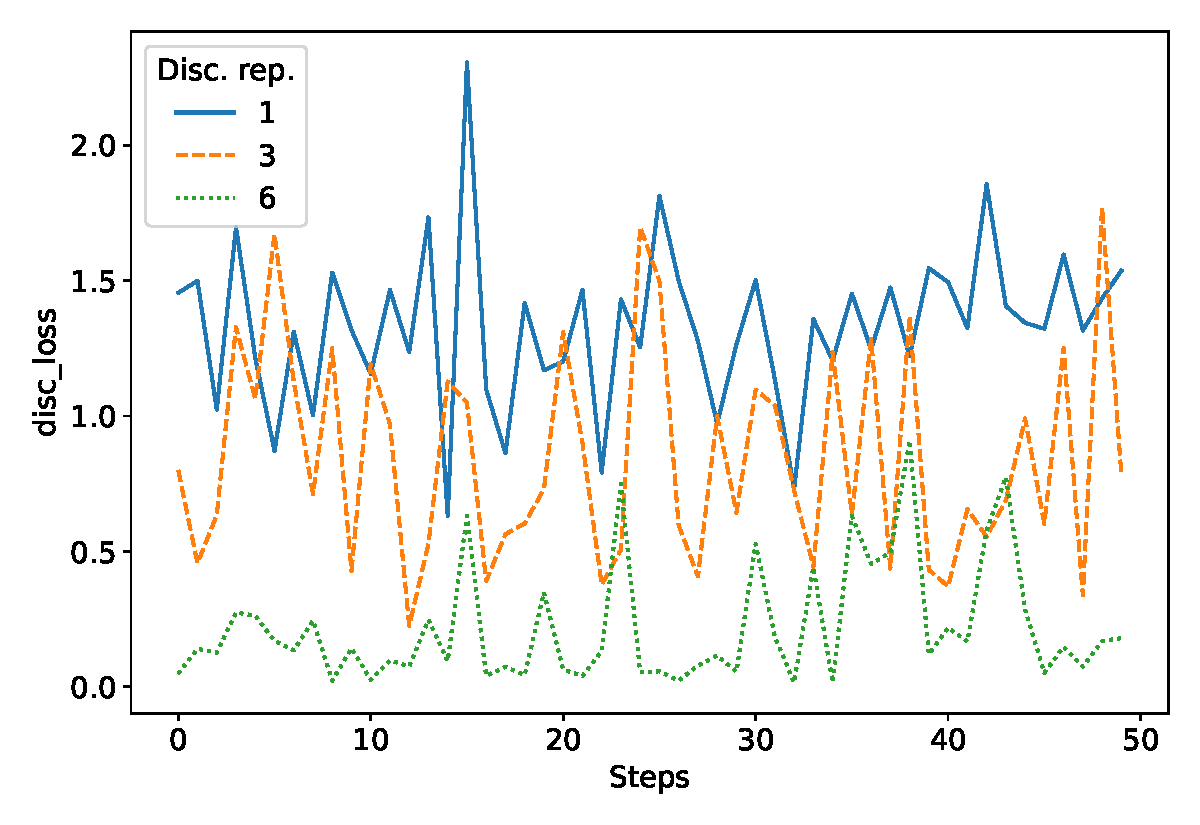
\includegraphics[width=\textwidth]{fig/analysis/Plot_Disc_rep_disc_loss.pdf}
		\caption{Discriminator loss for different discriminator training.}
		\label{fig:Plot_discrep_discloss}
	\end{subfigure}\hfill
	\begin{subfigure}{0.5\linewidth}
		\centering
		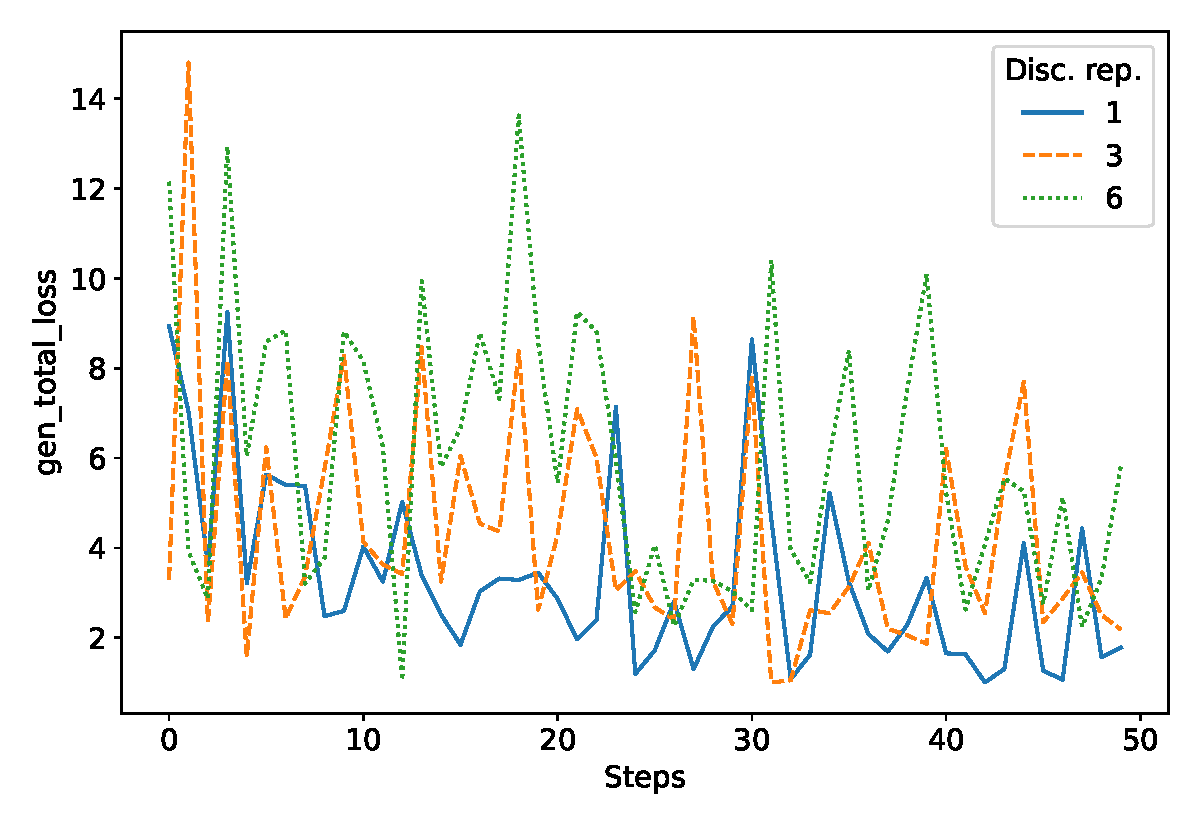
\includegraphics[width=\textwidth]{fig/analysis/Plot_Disc_rep_gen_total_loss.pdf}
		\caption{Generator losses for different discriminator training.}
		\label{fig:Plot_discrep_genloss}
	\end{subfigure}\hfill
	\caption{The amount of discriminator training has a high impact on the discriminator score. The discriminator repetition indicates the factor by which the discriminator is trained more with respect to the generator.}
	\label{fig:Plot_discrep_loss}
\end{figure*}
\begin{figure*}
	\centering
	\begin{subfigure}{0.5\linewidth}
		\centering
		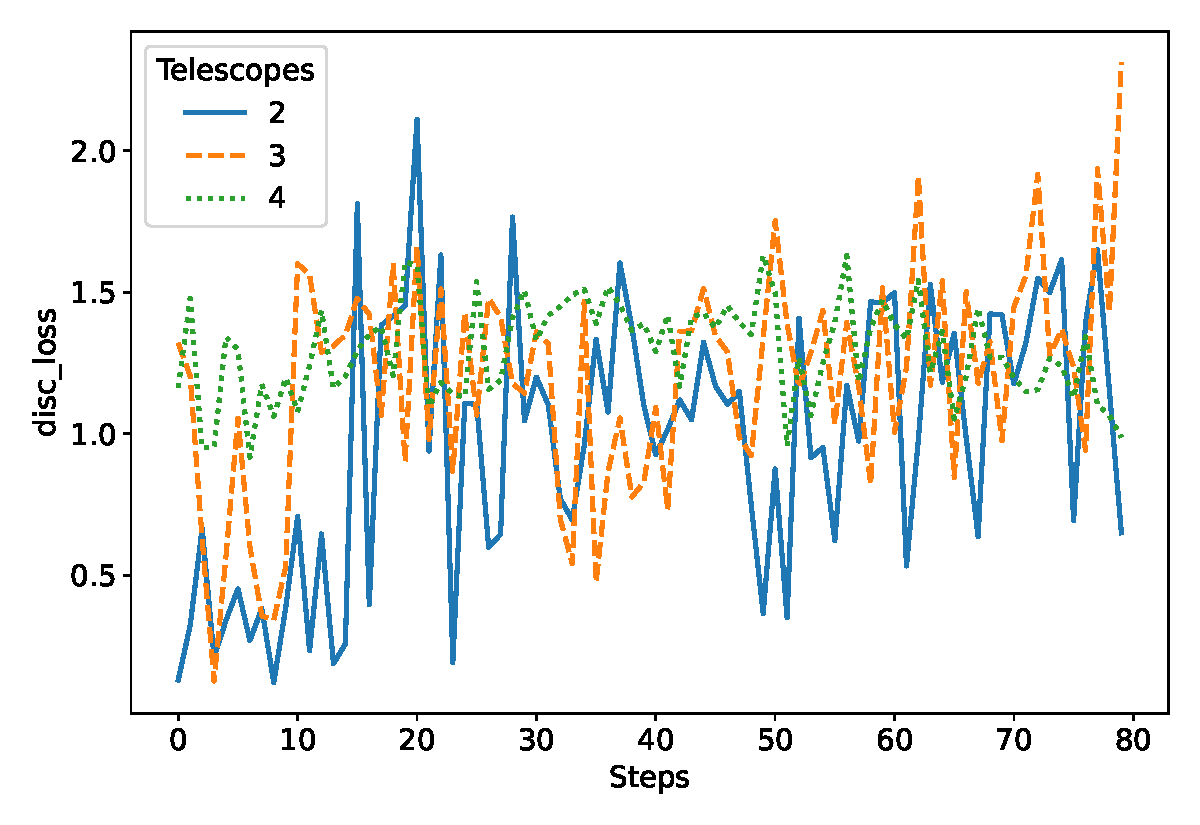
\includegraphics[width=\textwidth]{fig/analysis/Plot_N_telescopes_disc_loss.pdf}
		\caption{Discriminator loss for different amounts of telescopes.}
		\label{fig:Plot_telescopes_discloss}
	\end{subfigure}\hfill
	\begin{subfigure}{0.5\linewidth}
		\centering
		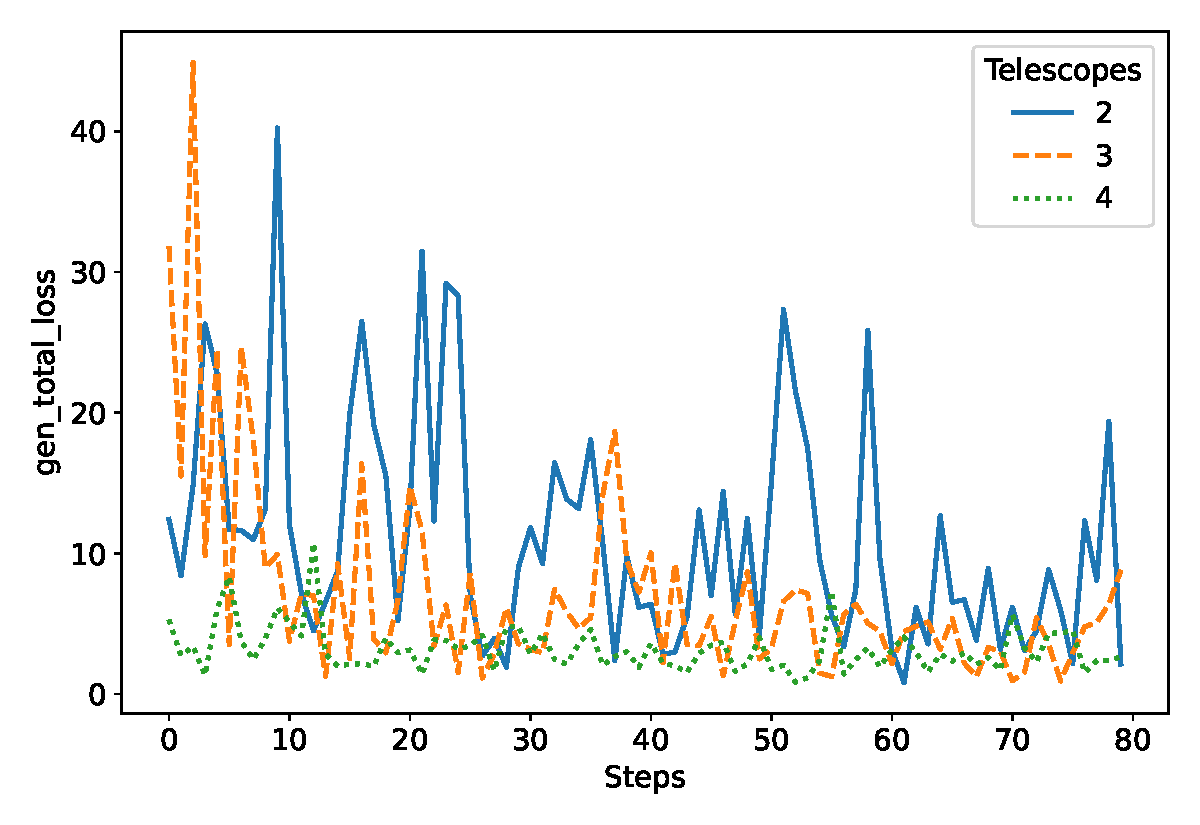
\includegraphics[width=\textwidth]{fig/analysis/Plot_N_telescopes_gen_total_loss.pdf}
		\caption{Generator loss for different amount of telescopes.}
		\label{fig:Plot_telescopes_genloss}
	\end{subfigure}\hfill
	\caption{The number of telescopes has a very impact on the model performance. If there are only two telescopes (1 baseline), both discriminator and generator are not trained smoothly: One gains a big advantage over the other. The result of four telescopes (6 baselines) is a lot better because the loss functions change only slightly with increasing steps.}
	\label{fig:Plot_telescopes_loss}
\end{figure*}
Later, GAN extended its version to a conditional model \citep{mirza2014conditional}. In this case, both generator and discriminator receive extra information $y$, such that the value function of the conditional GAN (cGAN) can be expressed as:
\begin{equation}
	\centering
	\begin{aligned}
		V(D, G) &= \mathbb{E}_{x \sim p_{data}(x)} \left[ \log D(x|y) \right] \\
		&+ \mathbb{E}_{z \sim p_{z}(z)} \left[ \log \left( 1-D(G(z|y) \right) \right]
	\end{aligned}
	\label{eq:conditional_GAN}
\end{equation}

Furthermore, \cite{isola2017image} observed that combining the cGAN given in equation \ref{eq:conditional_GAN} with the traditional L1-loss improves results, as the generator tries to be close to the ground truth. Hence, the function that is minimized as:
\begin{equation}
	\centering
	L_{tot} = \arg \min_{G} \max_{D} V(D, G) + \lambda \cdot L_1(G)
	\label{eq:total_gen_loss}
\end{equation}
where $\lambda$ = 100 and $L_1(G)$ is given as
\begin{equation}
	\centering
	L_1(G) = \mathbb{E}_{x,y,z} \left[ ||{y - G(x,z)}||_1 \right]
	\label{eq:l1_loss}
\end{equation}

This type of network is shown to be very robust, as it has been applied to several problems. Examples include creating colored images from grayscale images based on architectural labels, changing from day to night in different pictures, and predicting a map based on satellite data. A longer list of applications is given in \cite{isola2017image}. 


\subsection{Generator}
The used generator in this paper is a common U-Net convolutional network \citep{ronneberger2015u}. It consists of a contracting part, reducing the image size, and an expansive part, where the image is enlarged. The contracting part consists of repeated application of alternating convolutional layers and rectified linear unit (ReLU) layers. The expansion consists of repeated convolution, batch normalization, and ReLU layers. The first contracting step also includes a dropout layer \citep{isola2017image}.

\subsection{Discriminator}
The discriminator that has been taken here, named PatchGAN, does not work globally but rather classifies single patches as real or fake. The overall result is then estimated based on the average. The model architecture is as follows: zero padding, convolution, batch-norm, ReLu, zero-padding, and convolution \citep{isola2017image}.